\documentclass[a4paper,14.5pt,reqno]{amsart}
%\usepackage{times} % Basic Times font
%\usepackage{mathpazo} % Palatino text with math support
%\usepackage{charter}

\usepackage{subfiles}

\usepackage{xcolor}
\usepackage{graphicx}
\usepackage{amsmath}
\usepackage{libertinus}
\usepackage{natbib}
\bibliographystyle{plain}
\usepackage{blindtext}
\usepackage{graphicx}
\usepackage{thmtools}
\usepackage{cancel}
\usepackage[english]{babel}
\usepackage{amsthm}
\usepackage{mathrsfs}  
\usepackage{amsfonts}
\usepackage{amssymb}
\usepackage{amsmath}
\usepackage{bm}
\usepackage{bbm}
\usepackage[utf8]{inputenc}
\usepackage{blindtext}
%\usepackage{titlesec}
\usepackage{mathabx}
\makeatletter
%\renewcommand{\@secnumpunct}{.\quad}
\makeatother
\newcommand{\longrightharpoonup}{\relbar\joinrel\rightharpoonup}
\usepackage{harpoon}% <---


\usepackage{pgfplots}
\usepackage{tikz}
\usepackage{tikz-3dplot}
\usepgfplotslibrary{patchplots}

\theoremstyle{definition} % Ensures normal (upright) text inside the theorem

\newtheorem*{customthm}{} % Unnumbered theorem, no default label

\newenvironment{namedthm}[1]{%
    \smallskip % Adds space before the theorem
    \noindent\textbf{#1.} % No indentation, no auto punctuation, controlled spacing
}{%
    \par % Ensures proper paragraph formatting
}

\usepackage[dvipsnames]{xcolor}  % allows named colors like "blue", "magenta"
\usepackage{hyperref}

\hypersetup{
    colorlinks,       % disable colored text, use boxes
    %linkbordercolor = Cyan,   % color of internal document links
    %urlbordercolor = Melon, % color of external URL links
    %citebordercolor = NavyBlue,  % color of citation links
    %pdfborder = {0 0 1},      % thickness of link border
    linkcolor={black!50!black},
    citecolor={black!50!black},
    urlcolor={blue!50!black}
}

\usepackage[a4paper, total={6in, 8in}]{geometry}
\usepackage{algorithm}
\usepackage{algorithmic}

\usepackage{pgfplots}
\pgfplotsset{compat=1.18}

\usepackage{xcolor}


\newcommand*\de{\mathop{}\!\mathrm{d}}
\usepackage[thinc]{esdiff}

%\renewcommand*{\thefootnote}{\fnsymbol{footnote}}

\newcommand{\1}{\mathbbm{1}}
\DeclareMathOperator*{\argmin}{arg\,min}
\DeclareMathOperator*{\argmax}{arg\,max}
\DeclareMathOperator*{\supp}{supp}

\DeclareMathOperator{\imm}{Im}
\DeclareMathOperator{\lalpha}{\overline{\alpha}}
\DeclareMathOperator{\aconv}{\alpha\textit{x}+\overline{\alpha}\textit{y}}
\DeclareMathOperator{\bconv}{\beta\textit{x}+\overline{\beta}\textit{y}}


\theoremstyle{definition}
\newtheorem{definition}{Definition}[section]
\newtheorem{proposition}[definition]{Proposition}
\newtheorem{theorem}[definition]{Theorem}
\newtheorem{corollary}[definition]{Corollary}
\newtheorem{lemma}[definition]{Lemma}

\theoremstyle{remark}
\newtheorem*{example}{Example}
\newtheorem*{remark}{Remark}


\title{Information Geometry}
\author{Entropic Smash}
%\date{March 2025}

\begin{document}
\begin{figure}[t]
\begin{centering}
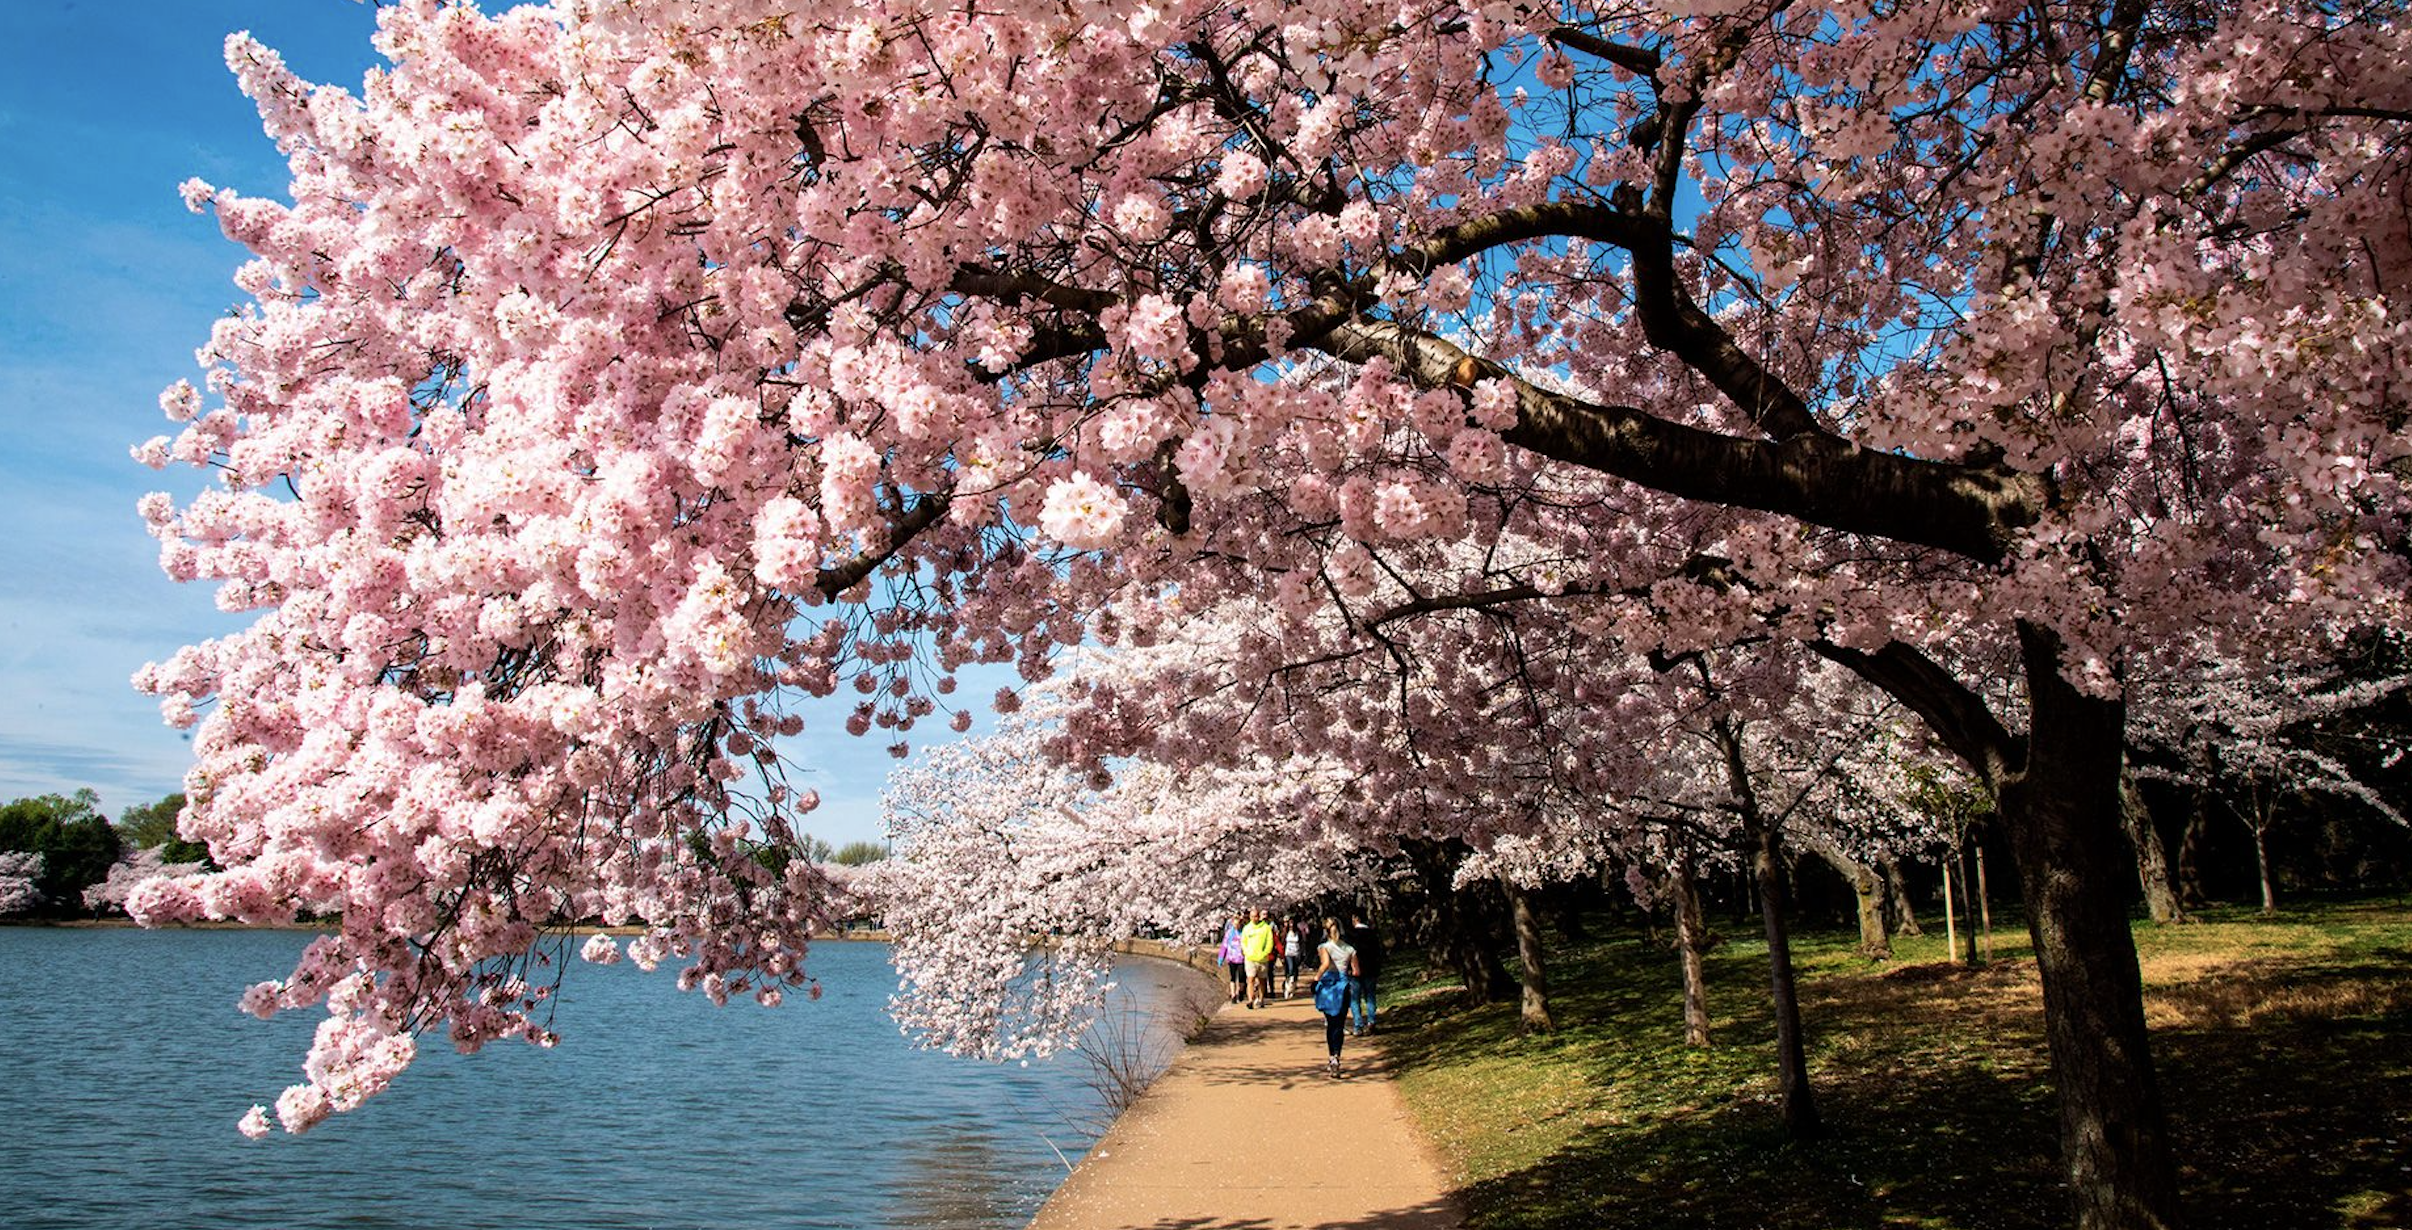
\includegraphics[scale=0.2]{images/Screenshot 2025-03-26 at 09.00.19.png}
\end{centering}
\end{figure}
\maketitle

\tableofcontents

\section{Introduction}
\subfile{Martucci/intro.tex}
\subsection{Obtaining tensors from $f$-divergences}
As S. Amari states, ``information geometry has emerged from studies of invariant geometrical
structure involved in statistical inference''.
In this section we link together some concepts introduced above, mainly showing that the choices of $g$ and $T$ are motivated by their property of invariance. Indeed, these metrics can be derived from an $f$-divergence, which is invariant. %da capire meglio

Consider the map we previously defined
\[
\Theta \ni \theta \mapsto  p_\theta \in \mathcal M
\]
and a convex, positive function $f$ such that $f(1)=0$. Then, the \textit{f-divergence} between two maps $p_\theta$ and $p_{\theta^{\prime}}$ is:
\[
D_f (p_\theta, p_{\theta^{\prime}}) = \int_{\Omega} f \bigg(\frac{p_\theta}{p_{\theta^{\prime}}}\bigg)p_{\theta^{\prime}} \,\,d{\mu}
\]

We want to look at curves $\theta:I\to\Theta$ parametrized by $t$ on the parameter space $\Theta$, and consider $\theta = \theta(t) $ and an increment along the curve $ \theta^{\prime}=\theta(t+h)$. We can compute the divergence between the distributions at these two values, namely $D_f (p_\theta, p_{\theta^{\prime}})$. \\Our question is: what happens if the increment $h$ is very very little?
That is, what happens if we Taylor expand the divergence $D_f$? \\
Of course, the 0-th order term is 0. It turns out that the first-order term is 0 as well, and the first meaningful terms are the second-order term, which depends on the Fisher information $g$ and on $f$ only by a number, and the third-order term, which depends on the 3-tensor $T$.   
\\
Let us compute this surprising result. 
%computations
Looking at the first-order term we have:
\[
\begin{aligned}
    &\frac{d}{dh} D_f(p_{\theta(t)}, p_{\theta(t+h)}) = \int \frac{d}{dh} p_{\theta (t+ h)} f\Bigl(\frac{p_{\theta(t)}}{p_{\theta(t+h)}}\Bigr)\, d\mu - \int p_{\theta(t+h)} f^{\prime}\Bigl(\frac{p_{\theta(t)}}{p_{\theta(t+h)}}\Bigr) \frac{p_{\theta(t)}}{p{^2}_{\theta(t+h)}} \frac{d}{dh}p_{\theta(t+h)} \, d\mu
\end{aligned}
\]
Now, evaluating this at $h=0$, in the second term we get $f'(1)$ evaluated at $h$, which is 0, bringing the whole term to 0; in the first term we exchange the integral and the derivative and get $\frac{d}{dh} \int p_{\theta(t)} \, d\mu = 0$ as the integral of a density function is equal to 1. Hence, the whole term goes to 0. \\
Let us look at the second-order term:
\[
\begin{aligned}
   \frac{d^2}{d^2h} D_f(p_{\theta(t)}, p_{\theta(t+h)}) &=  \frac{d}{dh}\int \frac{d}{dh} p_{\theta (t+ h)} f\Bigl(\frac{p_{\theta(t)}}{p_{\theta(t+h)}}\Bigr)\, d\mu - \frac{d}{dh}\int f^{\prime}\Bigl(\frac{p_{\theta(t)}}{p_{\theta(t+h)}}\Bigr) \frac{p_{\theta(t)}}{p_{\theta(t+h)}} \frac{d}{dh}p_{\theta(t+h)} \, d\mu \\&= -\int \Bigl(\frac{d}{dh} p_{\theta(t+h)}\Bigr)^2 f^{\prime} \Bigl(\frac{p_{\theta(t)}}{p_{\theta(t+h)}}\Bigr) \frac{p_{\theta(t)}}{p{^2}_{\theta(t+h)}} \, d\mu\, \\
   +\int \Bigl(\frac{d}{dh}& p_{\theta(t+h)}\Bigr)^2 \Biggl[f^{\prime\prime} \Bigl(\frac{p_{\theta(t)}}{p_{\theta(t+h)}}\Bigr) \frac{p_{\theta(t)}}{p_{\theta(t+h)}} \frac{p_{\theta(t)}}{p{^2}_{\theta(t+h)}} \frac{d}{dh} p_{\theta (t+ h)}
    + f^{\prime} \Bigl(\frac{p_{\theta(t)}}{p_{\theta(t+h)}}\Bigr)  \frac{p_{\theta(t)}}{p{^2}_{\theta(t+h)}}\frac{d}{dh} p_{\theta (t+ h)}\Biggr]\, d\mu \\
    &= \int \Bigl(\frac{d}{dh} p_{\theta(t+h)}\Bigr)^2 f^{\prime\prime} \Bigl(\frac{p_{\theta(t)}}{p_{\theta(t+h)}}\Bigr)  \frac{p{^2}_{\theta(t)}}{p{^3}_{\theta(t+h)}} \, d\mu\\
\end{aligned}
\]
Where between the first and second line we evaluate the two derivatives of a product only when the derivative doesn't fall at $\frac{d}{dh} p_{\theta(t)}$ because we already now it goes to 0 for $h=0$; then, between the second and forth line we have a nice cancellation and we are left only with one term of the sum. 
Evaluating this at $h=0$, we are left with:
\[
\begin{aligned}
\frac{d^2}{d^2h} D_f(p_{\theta(t)}, p_{\theta(t+h)})\Biggr|_{h=0} &= f^{\prime\prime} (1) \int \Bigl(\frac{d}{dh} p_{\theta(t)}\Bigr)^2 \frac{1}{p_{\theta(t)}} \, d\mu \\
&= f^{\prime\prime}(1) \int  \frac{\frac{d}{dt}p_{\theta(t)}}{p_{\theta(t)}}\frac{\frac{d}{dt}p_{\theta(t)}}{p_{\theta(t)}} p_{\theta(t)} d\mu \\
&= f^{\prime\prime}(1) \int  \frac{d}{dt} \log [p_{\theta(t)}] \frac{d}{dt} \log [p_{\theta (t)}]\,p_{\theta(t)} d\mu \\
&= f^{\prime\prime} (1)\, g(\gamma^., \gamma^.) 
\end{aligned}
\]
Where at this point we can equivalently evaluate the derivative at $t$, we multiply above and below by $p_{\theta(t)}$ and use the derivative of the log $\frac{d}{dt} \log p_{\theta(t)} = \frac{1}{p_{\theta(t)}} \frac{d}{dt} p_{\theta(t)}$.
We get a term depending only on a constant $f(1)$ and the Fisher information $g$ evaluated at a very specific derivative, which is the derivative along the curve, which is nothing but the velocity of the curve. 

Now, turn to the third-order term, we have to take the derivative of what we found above:
\[
\begin{aligned}
    \frac{d^3}{d^3h} D_f(p_{\theta(t)}, p_{\theta(t+h)}) &= \frac{d}{dh} \int \Bigl(\frac{d}{dh} p_{\theta(t+h)}\Bigr)^2 f^{\prime\prime} \Bigl(\frac{p_{\theta(t)}}{p_{\theta(t+h)}}\Bigr)  \frac{p{^2}_{\theta(t)}}{p{^3}_{\theta(t+h)}} \, d\mu\\
    &=\int\frac{d}{dh}\Biggl[\Bigl(\frac{d}{dh} p_{\theta(t+h)}\Bigr)^2 f^{\prime\prime} \Bigl(\frac{p_{\theta(t)}}{p_{\theta(t+h)}}\Bigr)  \frac{p{^2}_{\theta(t)}}{p{^3}_{\theta(t+h)}}\Biggr]  \, d\mu\\
    &=\int \frac{d}{dh} \Bigl[ f^{\prime\prime} \Bigl(\frac{p_{\theta(t)}}{p_{\theta(t+h)}}\Bigr) \frac{p{^2}_{\theta(t)}}{p{^3}_{\theta(t+h)}}\Bigr] \Bigl(\frac{d}{dh} p_{\theta(t+h)} \Bigr)^2 + \frac{d}{dh}\Bigl[ \Bigl(\frac{d}{dh} p_{\theta(t+h)}\Bigr)^2 \Bigr] f^{\prime\prime} \Bigl(\frac{p_{\theta(t)}}{p_{\theta(t+h)}}\Bigr)  \frac{p{^2}_{\theta(t)}}{p{^3}_{\theta(t+h)}}\, d\mu
\end{aligned}
\]


Let's compute the first term, when the derivative falls on $f^{\prime\prime} \bigl(\frac{p_{\theta(t)}}{p_{\theta(t+h)}}\big) \frac{p{^2}_{\theta(t)}}{p{^3}_{\theta(t+h)}}$.
\[
\begin{aligned}
    \int\biggl(\frac{d}{dh} p_{\theta(t+h)}\biggr)^2 \Biggl[- f^{\prime\prime\prime}\biggl(\frac{p_{\theta(t)}}{p_{\theta(t+h)}}\biggr) \frac{p_{\theta(t)}^3}{p_{\theta(t+h)}^5} \frac{d}{dh}p_{\theta(t+h)} - 3f^{\prime\prime}\biggl(\frac{p_{\theta(t)}}{p_{\theta(t+h)}}\biggr) \frac{p_{\theta(t)}^2}{p_{\theta(t+h)}^4} \frac{d}{dh}p_{\theta(t+h)} \Biggr] \, d\mu 
\end{aligned}
\]
Evaluating it at $h=0$:
\[
\begin{aligned}
    &\int\Bigl(\frac{d}{dt} p_{\theta(t)}\Bigr)^3  \Bigl(- f^{\prime \prime \prime} (1) \frac{1}{p{^2}_{\theta(t)}} - 3f^{ \prime \prime} (1) \frac{1}{p{^2}_{\theta(t)}}\Bigr) \,\, d\mu  \\
    &=- \bigl(f^{\prime \prime \prime} (1) +3 f^{\prime \prime} (1)\bigr)\int \Bigl(\frac{d}{dt} p_{\theta(t)}\Bigr)^3\frac{1}{p{^2}_{\theta(t)}} \,\, d\mu \\
\end{aligned}
\]
And using the same trick as above we get:
\[
\begin{aligned}
     &= - \bigl(f^{\prime \prime \prime} (1) +3 f^{\prime \prime} (1)\bigr) \int\frac{d}{dt} \log p_{\theta(t)}\frac{d}{dt} \log p_{\theta(t)}\frac{d}{dt} \log p_{\theta(t)}\,\, p_{\theta(t)}\, d\mu \\
    &=- \bigl(f^{\prime \prime \prime} (1) +3 f^{\prime \prime} (1)\bigr) \, T(\gamma ^.,\gamma ^.,\gamma ^.)
\end{aligned}
\]
i.e., we get exactly a term depending on the Amari-Chentsov tensor evaluated at $\gamma^.$\\

Now, let's go back and analyze the case when the derivative falls on $\bigl(\frac{d}{dh} p_{\theta(t+h)}\bigr)^2$:
\[
\begin{aligned}
    & \int\frac{d}{dh} \biggl(\frac{d}{dh} p_{\theta(t+h)}\biggr)^2 f^{\prime\prime}\biggl(\frac{p_{\theta(t)}}{p_{\theta(t+h)}}\biggr)\frac{p{^2}_{\theta(t)}}{p{^3}_{\theta(t+h)}} \, \, d\mu \\
\end{aligned}
\]
Evaluating this term at $h=0$ we get:
\[
\begin{aligned}
        &=2 \int\frac{d}{dt} p_{\theta(t)} \frac{d^2}{d^2t} p_{\theta(t)} f^{\prime\prime} (1) \frac{1}{p_{\theta(t)}} \, \, d\mu \\
        &= 2f^{\prime\prime} (1)  \int\frac{d}{dt} \log p_{\theta(t)} \frac{d^2}{d^2t} p_{\theta(t)} \, \, d\mu 
\end{aligned}  
\]
Aaaaaand bo :) [...]\\

Overall, the cool result we get is that Taylor expanding the f-divergence along a curve $\gamma$ on the parameter space $\Theta$, the first significant terms we get are exactly the Fisher-Rao metric $g$ and the Amari-Chentsov $T$ evaluated at the derivative along the curve. 
%\include{matilde}
\section{Fundamental concepts in geometry}

$\cdot$ This is the 2nd reading seminar of the series, held by Prof. Pigati on April 1st $\cdot $\\

What follows is a set of informal definitions of objects like manifolds, charts and tangent space that are at the basis of the geometric framework introduced above. 

Given $n \in \mathbb{N}$, a n-dimensional \textit{manifold} $\mathcal{M}^n$ is, roughly, something that looks like the Euclidean space $\mathbb{R}^n$ at small scale. When defining manifolds, we don't actually use a notion of distance (metric), instead we use topological notions and define a ``small scale" in terms of open sets. 

\begin{definition}[Manifold] \label{def:mnf}%or structure of manifold? 
    Given a topological space $M^n$ (Hausdorff*, second countable), a structure of an n-dimensional manifold is given by:
    \begin{itemize}
        \item[i.] a collection $\{U_i\}_{i \in I}$ of open sets $U_i \subseteq M$ such that $M= \bigcup_{i \in I} U_i$;
        \item[ii.] for each $i$, a bijective map $\varphi_i : U_i \longrightarrow V_i \subseteq \mathbb{R}^n$;
        \item[iii.] $\varphi_i \circ \varphi^{-1}_j : \varphi_j (U_i \cap U_j) \longrightarrow \varphi_i(U_i \cap U_j)$ is $C^\infty$ \,\,\,\, \textit{(compatibility property)}
    \end{itemize}
    Where you can think of the property of being ``Hausdorff" as the points in the space being distinguishable; and the compatibility property ensures we can define what is a smooth function on our manifold. \\

\end{definition}

\begin{example}
    Take $U\subset \mathbb{R}^n$ open. $\mathcal{M}^n := U$ is a n-dimensional manifold with open cover $\{U\}$ and chart $\{id: U\longrightarrow U\}$.
\end{example}

\begin{example}\label{ex:sn_1}
    Take the unitary n-dimensional sphere $S^n = \{x \in \mathbb{R}^{n+1}:|x| = 1\}$. Given $p \in S^n$, we define the emisphere related to $p$ by cutting the sphere in half with the hyperplane generated by the vector $p$ (the hyperplane orthogonal to it) where the origin $0$ lies, i.e. $U_p := \{x \in S^n : (x,p)>0\}$. Then, $\varphi_p:U_p \longrightarrow B_1(0)$ is a projection that ``flattens" the emisphere onto the hyperplane. 
\end{example}

\begin{example}[Guess the manifold]\label{ex:cyl}
    Take $M^2= U_1 \cup U_2$.\\
    $\varphi_1: U_1 \longrightarrow \mathbb{R} \times (0, 2\pi)$\\
    $\varphi_2: U_2 \longrightarrow \mathbb{R} \times (0, 2\pi)$\\
    $\varphi_1(U_1 \cap U_2) = \mathbb{R}\times (\pi, 2\pi)$\\
    $\varphi_2  \circ \varphi_1^{-1}(x,y) := (x, y-\pi)$\\
    
    \textbf{Solution:} We can deduce that our manifold $M$ is a cylinder. The charts $\varphi_1$ and $\varphi_2$ will be maps from the manifold to the cylinder minus one line (to ensure bijection). %si?
\end{example}

\begin{example}[Guess the manifold]\label{ex:sn_2}
    Take $M^2= U_1 \cup U_2$.\\
    $\varphi_1: U_1 \longrightarrow \mathbb{R}^2 $\\
    $\varphi_2: U_2 \longrightarrow \mathbb{R}^2$\\
    $\varphi_1(U_1 \cap U_2) = \varphi_2(U_1 \cap U_2) = \mathbb{R}^2 \setminus \{0\}$\\
    $\varphi_2  \circ \varphi_1^{-1}(x) = \frac{x}{|x|^2}$\\
    
    \textbf{Solution:} We can deduce that our manifold is the 2-dimensional sphere $S^2$, where $\varphi_1 $is given by the sphere without the point at the north pole, and $\varphi_2$ is given by removing the south pole. The two maps project the manifold onto the plane cutting it in half (the plane where the equator lies). 
\end{example}

\begin{definition}[Charts]
    The maps $\varphi_i:U_i \longrightarrow V_i$ used in definition \ref{def:mnf} are called charts. The inverse maps $\varphi_i^{-1}$ are called parametrizations. 
\end{definition}

    The main conceptual idea is that for any point $x \in M^n$ in the manifold, you can find an open set $U_i$ that is omeomorphic to an open subset of the Euclidean space $\mathbb{R}^n$. Figure \ref{fig:mnf} helps visualizing this idea. 
    Then, we can think of charts as maps allowing us to find (multiple sets of) ``coordinates" for points on the manifold. Indeed, the inverse of a chart is a parametrization in the sense that it maps some parameters - vectors in $\mathbb{R}^n$ - to points in our manifold. What we hope is that the combination of charts defined on the same region on the manifold is smooth (compatibility property), in order to define a \textit{smooth} manifold (we could hope for any other property like continuity or $C^7$, and to enforce it we would impose it on charts in the same way). 


\begin{definition}[Atlas and maximal atlas]
A collection of charts is called an \textit{atlas}. Any atlas can be uniquely extended to a maximal atlas, which is one that is not contained in any other atlas.
\end{definition}

\begin{remark}
    Recall the examples above: the two structures we have defined on the manifold $S^n$ are the same, i.e. they give the same maximal atlas. 
\end{remark}

\begin{example}
    Here's instead an example of incompatible charts. Take $M=\mathbb{R}$ and the charts $id:M\longrightarrow \mathbb{R}$ and $\psi: M\longrightarrow \mathbb{R} : \psi(x)=x^3$. Then we get $id \circ \psi^{-1}(x) = \sqrt[3]{x} \notin C^\infty.$
\end{example}

\begin{definition}[Smoothness]
    Let $M,N$ be two manifolds such that:
    \begin{itemize}
        \item[] $M$ has atlas $\{\varphi_i\}_{i\in  I}:U_i \longrightarrow \mathbb{R}^n$
        \item[] $N$ has atlas $\{\psi_j\}_{j\in  J}:V_j\longrightarrow \mathbb{R}^n$
    \end{itemize}
    Given $p\in M$, $f:M \longrightarrow N$ is smooth if $\exists U_i \ni p$ and $\exists W_j \ni f(p), W_j \subseteq \mathbb{R}^n,$ such that the map
    \[\psi_j \circ f \circ \varphi_i^{-1}: \varphi_i(f^{-1}(W_j)) \longrightarrow W_j\] %i'm not sure it should be W_j here but rather psi(Wj)
    is smooth.\\
    Moreover, using compatibility of charts we can replace ``$\exists$" with ``$\forall$".
\end{definition}

Now, we turn to defining  what a tangent space is. approximated to a tangent space. 


\begin{figure}
    \centering
    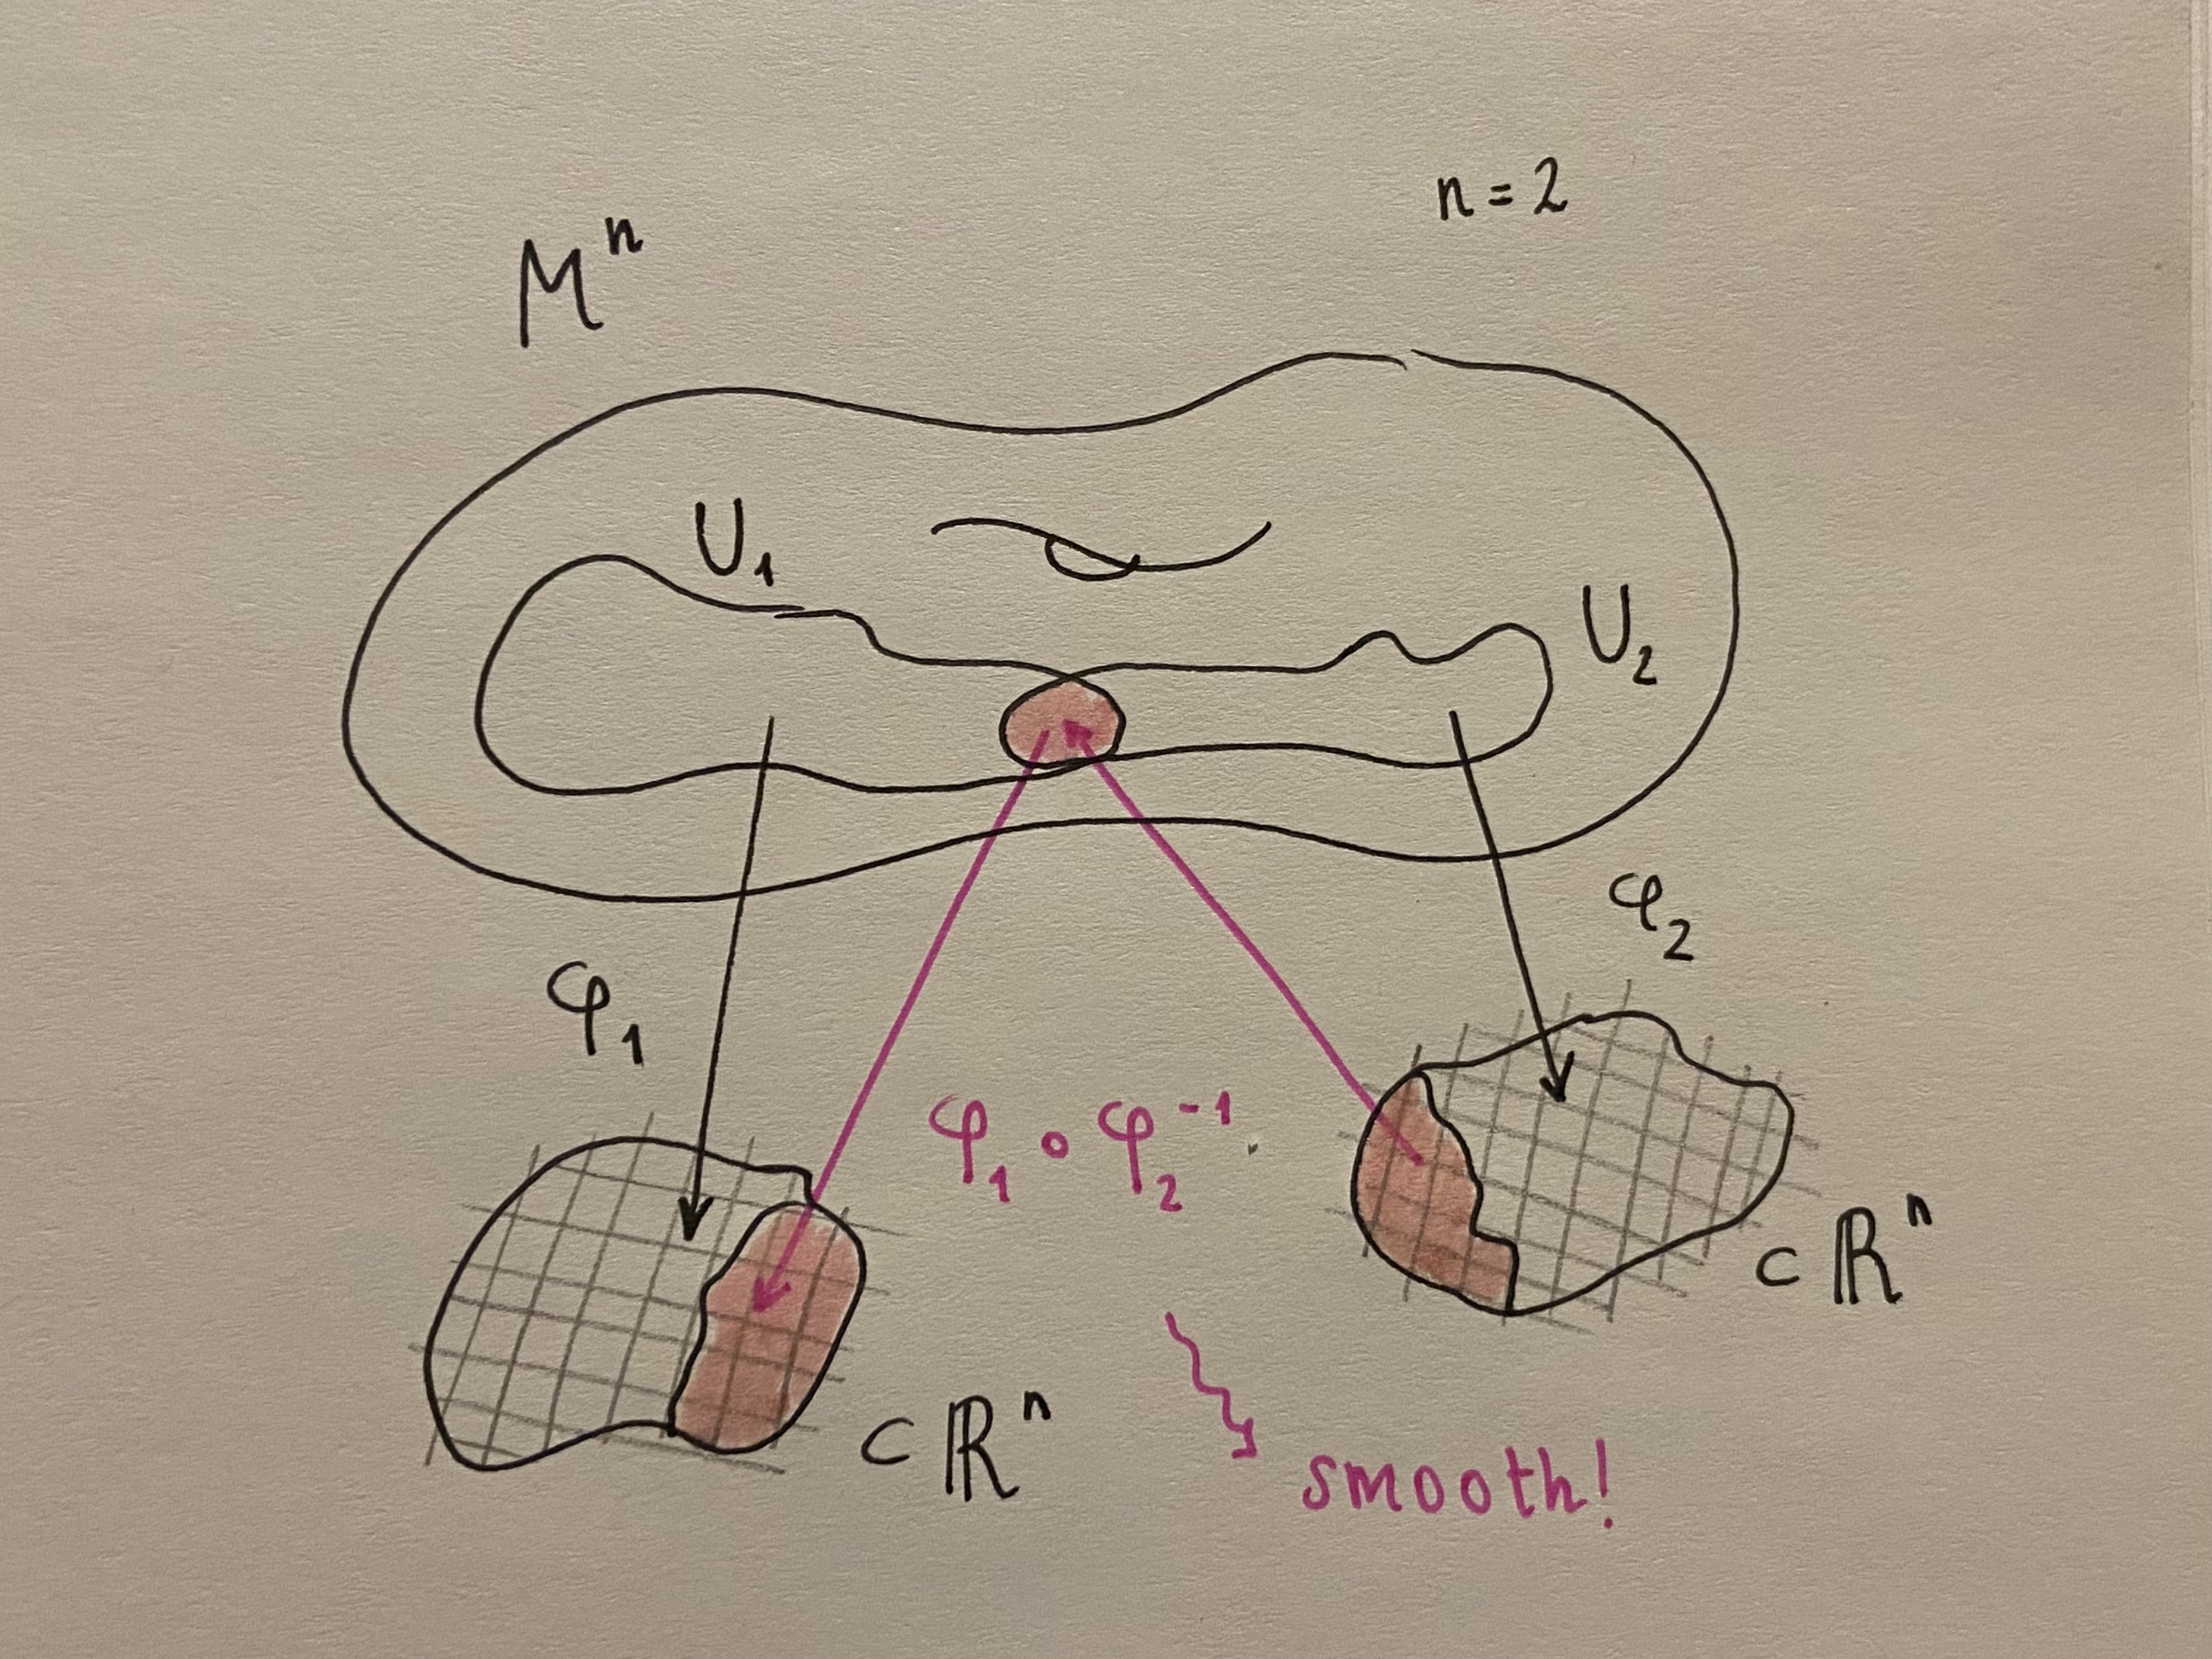
\includegraphics[width=0.5\linewidth]{images/manifold.png}
    \caption{Visual representation of a manifold. The two sets in the lower part are subsets of the Euclidean space, i.e. charts. What you would like is that the pink map ($\varphi_2  \circ \varphi_1^{-1}$) is smooth, so that the two coordinate system defined on the pink region of the manifold ($U_1 \cap U_2$) are compatible.}
    \label{fig:mnf}
\end{figure}
\subsection{Tangent spaces}
We can get an intuition of \textit{tangent spaces} by means of a useful analogy. Just like we can approximate a smooth function to a linear one, by taking its Taylor expansion, any manifold can be approximated to a tangent space. 

Let $p \in M^n$. If $n=0$ we simply define $T_pM \coloneq \{0\}$. Now, assume $n>0$. We give two possible definitions of the tangent space at $p$ and we will later comment on their equivalence. The first one is more visual, you think of vectors in the tangent space as velocities of curves starting at $p$. The second approach is more algebraic, you think of the tangent space as all the possible ways to perform a directional derivative of a function. 

\bigskip
\emph{First approach (visual)}: Consider the space of all smooth curves $\gamma: [0, \varepsilon] \to M$, $\gamma(0)=p$ starting from $p$. We declare two such curves equivalent if their velocity is equal when read in every chart. Formally, for any $\gamma_1: [0, \varepsilon_1] \to M$ and $\gamma_2: [0, \varepsilon_2]\to M$, $\gamma_1 \sim \gamma_2$ if for any chart $\varphi: U \to V \subseteq \mathbb{R}^n$  around $p$, it holds $(\varphi \circ \gamma_1)'(0) = (\varphi \circ \gamma_2)'(0)$. Then $T_pM$ will be defined as the set of all equivalence classes.

A few remarks are in order. 

\begin{remark}
    It is enough to check the condition in the definition only for one chart. Indeed, when changing chart, the velocity is transformed by applying the differential of the change of chart map (which we recall to be smooth by the definition of smooth manifold).
\end{remark}

\begin{remark}
    $T_pM$ is indeed a vector space and its dimension is the same as the one of the manifold. To see this, fix any chart centered at $p$ (we can always choose such a chart up to translation and moreover the choice is irrelevant by the previous remark) $\varphi:U \to V$ with $p \in U$ and consider for any $w \in \mathbb{R}^n$ the curve $\gamma_w(t) \coloneq \varphi^{-1}(tw)$, that is, the preimage through the chart of the line spanned by $w$ in $\mathbb{R}^n$. One can show that the map $w \mapsto [\gamma_w]$ is a bijection between $\mathbb{R}^n$ and $T_pM$. The sum operation on the equivalence classes is then defined by $[\gamma_w]+[\gamma_v]\coloneq [\gamma_{w+v}]$. The vector space structure hereby defined does not depend on the choice of chart.
\end{remark}

\begin{remark}
    When the manifold is immersed in some Euclidean space $\mathbb{R}^n$, we can view $T_pM$ as a vector subspace. The affine subspace $p+T_pM$ corresponds to our intuition of a ``Taylor approximation" of $M$. For a surface (2-dimensional manifold) in $\mathbb{R}^3$ that would be the tangent plane to the surface. 
\end{remark}

\emph{Second approach (algebraic)
}: Consider the space of real valued smooth functions on M, denoted $C^{\infty}(M)$. We call a map $D: C^{\infty}(M) \to \mathbb{R}$ a \emph{derivation} at $p$ if it is linear and it satisfies the following product rule: $D(fg)=D(f)g(p)+f(p)D(g)$. Derivations are essentially directional derivatives of functions, evaluated at $p$. We define the tangent space as the set of all derivations at $p$, that is, all possible ways of performing a directional derivative of a function. 

\begin{remark}
    The vector space structure in this second definition is clearer (sums and scalar multiples of derivations are still derivations) but proving that it has dimension $n$ still requires some work. A possible strategy would be proving that, given a derivation $D$ at $p$ and a chart $\varphi:U\to V$ centered at $p$, there exists a vector $w \in \mathbb{R}^n$ such that $D(f)$ is the directional derivative of $f \circ \varphi^{-1}$ in direction $w$ evaluated at $0$. The proof of this fact uses the following factorization lemma:
    \begin{lemma}
        For any $f \in C^{\infty}(M), f(x) = f(0) + \sum_{i=1}^nx_ig_i(x)$ for some smooth functions $\{g_i\}$.
    \end{lemma}
\end{remark}

The connection between the two definitions is the following. Given an equaivalence class $[\gamma]$ as in the first definition, we get a derivation $D$ by defining $D(f) \coloneq (f \circ \gamma)'(0) \in \mathbb{R}$. Using local charts one can check that this is indeed a bijection.

\begin{example}
    Consider the sphere $S^n \subseteq \mathbb{R}^{n+1}$. It is conveniently defined as the zero set of a smooth function, namely $h(x) = |x|^2-1$. In such a case, one can show that the tangent space is the zero set of its differential:
    \begin{equation*}
        T_pS^n=\ker Dh(p)=\ker (v\mapsto2\langle p,v \rangle)
    \end{equation*}
    Hence, the tangent space to the sphere at $p$ is none other than the orthogonal complement $p^\perp$.
\end{example}

\subsection{Vector bundles}
We now turn to a different construction, ubiquitous in differential geometry, which is the one of vector bundles. Informally, they provide a smooth way to glue together different vector spaces at each point of a manifold. 

\begin{definition}[Vector bundle] \label{definition:vector bundle}
    Let $M$ be an n-dimensional manifold and $k$ a positive integer. A \emph{vector bundle} of rank $k$ over $M$ is a manifold $E^{n+k}$ together with a smooth map $\pi:E \to M$, called projection, such that:
    \begin{enumerate}
        \item each fiber $E_p :=\pi^{-1}(p)$ has the structure of a $k$-dimensional vector space
        \item for each $p \in M$ there exists a neighborhood $U$ of $p$ and a diffeomorphism $\Phi: \pi^{-1}(U) \to \mathbb{R}^k \times U$, called \emph{local trivialization}, of the form $\Phi=(F, \pi)$, where $F$ is a vector space isomorphism with $\mathbb{R}^k$ when restricted to each fiber.     \end{enumerate}  
\end{definition}

Notice that in the definition above, we assumed a smooth structure on the total space $E$ as a datum. However, the way vector bundles arise in practice is from disjoint unions of vector spaces assigned to each point of the manifold. With this in mind, let us see a more operational, yet equivalent, characterization of vector bundles which gives a smooth structure on the total space almost for free, provided that the local trivializations overlap in a specific way.

\begin{proposition}
    Suppose that for each $p \in M$ we have a real vector space $E_p$ of some fixed dimension $k$ and let $E := \bigsqcup_{p \in M} E_p$. If moreover we have an open cover $\{U_\alpha\}_{\alpha \in A}$ of $M$ and a bijective map $\Phi_\alpha : \pi^{-1}(U_\alpha) \to \mathbb{R}^k  \times U_\alpha$ of the same form as in Definition \ref{definition:vector bundle} (ii) for each $\alpha \in A$ and if it holds that for each $\alpha, \beta \in A$ with $U_\alpha \cap U_\beta \neq \emptyset$, the map $\Phi_\alpha \circ \Phi_\beta^{-1}$ from $ \mathbb{R}^k \times (U_\alpha \cap U_\beta)$ to itself has the form
    \[
    \Phi_\alpha \circ \Phi_\beta^{-1}(v, p) = (L_pv, p)
    \]for some $L_p \in GL(k, \mathbb{R})$ depending smoothly on p, then $E$ has a unique topology and smooth structure making it into a smooth manifold and a smooth rank-$k$ vector bundle over $M$, with the obvious projection $\pi$ and $\{\Phi_\alpha\}$ as smooth local trivializations.
\end{proposition}

\begin{example} [Tangent Bundle]
    Denote $TM = \bigsqcup_{p \in M} T_pM$ and by $\pi$ the obvious projection. We want to put a structure of vector bundle of rank $2n$ on $TM$ which will then take the name of \emph{tangent bundle}. This is the prototypical example of a situation where we want to glue together different vector spaces, in this case the tangent spaces, at each point of $M$. In principle, we should construct a topology and a differentiable structure on $TM$, but using the equivalent characterization we just gave, we can bypass this step and directly provide the local trivializations and transition functions, which incidentally are fairly simple in this case. 

    Take a smooth atlas of M (to fix ideas you can take the maximal one) and in the domain of each chart define the map $\Phi: \pi^{-1}(U) \to \mathbb{R}^n \times U$ by
    \begin{equation*}
        \Phi\left(\sum_i v^i \left. \frac{\partial}{\partial x^i} \right|_p\right) := ((v^1,\dots,v^n),p)
    \end{equation*}
    where $\{\left. \frac{\partial}{\partial x^i} \right|_p\}$ is the basis of $T_pM$ induced by the coordinates of the chart. This is clearly bijective and restricts to a linear isomorphism with $\mathbb{R}^n$ on fibers. Finally, one can easily check that for any two such maps the transition function is given by the differential of the change of coordinates, which is indeed an invertible linear map:
    \begin{equation*}
        \Phi_\alpha \circ \Phi_\beta^{-1}(v, p) = (D(\varphi_\alpha\circ\varphi_\beta^{-1})(x)[v], p).
    \end{equation*}
\end{example}

We can define a suitable notion of \emph{isomorphism of vector bundles}

\begin{definition}
    We call two vector bundles $E, E'$ isomorphic if there exists a diffeomorphism $F: E \to E'$ that respects the fibers, that is $E_p$ goes to $E'_{F(p)}$, or more compactly $\pi_{E'}\circ F=\pi_E$, and gives a linear isomorphism on each fiber. Moreover we say that $E$ is \emph{trivial} if is isomorphic to $\mathbb{R}^k\times M$.
\end{definition}

\begin{example} [$TS^1$ is trivial]
    Recalling that the tangent space to a point on the sphere is its orthogonal complement we define the vector bundle isomorphism $F:\mathbb{R}\times S^1 \to TS^1$ by $F(t,p) = tRp \in T_pS^1$ where $R$ is a counterclockwise $90$ degrees rotation. 
\end{example}

\begin{remark}
    In light of this, we may hypothesize that the tangent bundle of any sphere is trivial. It turns out that it is not true and this fails already in dimension $2$. However, proving that $TS^2$ is not trivial requires a very deep theorem in differential topology, called the \emph{hairy ball theorem} which states that there is no nonvanishing smooth (actually continuous) tangent \emph{vector field} on even-dimensional n-spheres. The connection with triviality of vector bundles comes from the fact that being trivial is equivalent to having a smoothly varying choice of basis of each fiber. If this were the case on the $2-$sphere we would have a smooth nonvanishing vector field on it, thus contradicting the hairy ball theorem. 

    In full generality, $TS^n$ is trivial if and only if $n \in \{1,3,7\}$
\end{remark}

\begin{example} [$TS^3$ is trivial]
    To show this, it is convenient to view $S^3$ as a subset of the quaternions: $S^3 := \{a+ib+jc+kd | a^2+b^2+c^2+d^2=1\}$. The map $F:\mathbb{R}^3\times S^3 \to TS^3$ defined by \[ F((t_1,t_2,t_3),p) = t_1pi+t_2pj+t_3pk \in T_pS^3 \] for example, is a vector bundle isomorphism.
\end{example}
    




\section{Riemannian geometry}

Seminar 15 apr, Prof. Pigati. [Next meeting is May 13, then May 27 ]
% THERE IS NO AUDIO :((((
% connections 
% concepts in riem. geometry 

Connections:
a way to perform derivatives on a manifold

\begin{definition}[Section of a map] A smooth section $s:M \to E$ is a smooth map such that $s(p) \in \pi^{-1}(p) \,\, \forall p\in M$
\end{definition}
When $E = TM$, a section is called a vector field. 
(Recall $E$ is our vector bundle with associated map $\pi$, and $X=\sum_{i=1}^n X^i\frac{\partial}{\partial x_i}$.

\begin{definition}[Connection]
    A connection on $E$, denoted $\nabla$, takes a section $s$ of $E$ and a vector field $X$, and gives a new section $\nabla_Xs$ that satisfies the following properties:
\begin{itemize}
    \item $C^\infty(M)$-linear in $X$: $\nabla_{fX+gY} s=f\nabla_X s + g\nabla_Y s \quad \forall f,g: M \to \mathbb{R}$
    \item $\mathbb{R}$-linear in s
    \item Leibniz rule: $\nabla_X(fs) = f \nabla_x s + X(f) s$
\end{itemize}
Where $X(f)$ indicates differentiating $f$ along direction $X$.  
\end{definition}

\begin{remark}
    $\nabla_X s(p)$ depends only on $s|_U$ for an arbitrary small neighborhood $U$ and on $X(p)$.
\end{remark}

\begin{remark}
    In a trivialization $\pi^{-1} \cong \mathbb{R}^k \times U$ we always have the following structure:
    \[
    s(x) = (v(x), x)
    \]
    \[
    \nabla_X s(x) = Ds(x) [X(x)] + X^iA_i(x) s(x)
    \]
    Where $A$ is a $k\times k$ matrix, not necessarily invertible. 
\end{remark}

\begin{remark}
    If $\nabla$ is a connection, any other connection has the form $\tilde{\nabla} = \nabla + \alpha$ where $\alpha(x):\pi^{-1}(x) \otimes T_x^*M \to \pi^{-1}(x)$ is a linear map. Namely, $\tilde \nabla_X s = \nabla_X s + \alpha(X) s$, where $\alpha(X) s$ is the ``0-th order term". 
\end{remark}

Hence, the space of all connections is an \textbf{affine space}. 

In computations, assuming $U$ trivializes $E$ and is included in a chart, we can write \[\nabla_{\frac{\partial}{\partial x_i}}e_j= \sum_{l=1}^{\text{rank}} \Gamma_{ij}^l e_l\] where $\{e_1, \ldots, e_k\}$ is a canonical basis of $\mathbb{R}^k \cong \pi^{-1}(x)$. $\Gamma_{ij}^l (x)$ are called \emph{Christoffel symbols}. 

$A_i(x)$ has coefficient $\Gamma_{ij}^l $ in position $(l,j)$.

\[
\nabla_{\frac{\partial}{\partial x^i}}
\begin{pmatrix}
c_1(x)\\
\vdots\\
c_k(x)
\end{pmatrix}
=
\begin{pmatrix}
\frac{\partial c_1}{\partial x^i}\\[6pt]
\vdots\\[6pt]
\frac{\partial c_k}{\partial x^i}
\end{pmatrix}
\;+\;
A_i
\begin{pmatrix}
c_1(x)\\
\vdots\\
c_k(x)
\end{pmatrix}\,.
\]

\begin{remark}
    For $E=TM$ we just need to take $U$=domain of chart. Then $TM|_U$ is trivialized by $c_1(x)\frac{\partial}{\partial x^1} + \ldots + c_n(x)\frac{\partial}{\partial x^n}$ and $\nabla_{\frac{\partial}{\partial x^i}} (\frac{\partial}{\partial x^j}) = \sum_{l=1}^n \Gamma_{ij}^l \frac{\partial}{\partial x^l}$
\end{remark} 

\subsection{Parallel Transport}
Given a smooth curve $\gamma: [0, T] \to M$, a section along $\gamma$ is $s:[0,T] \to E$ (smooth) s.t. $s(t) \in \pi^{-1}(\gamma(t))$

\begin{example}
    Given any $v_0 \in \pi^{-1}(\gamma(0)$ there is a unique section $s(t)$ along $\gamma$ s.t. $\nabla_{\gamma'(t)} s(t) = 0.$ What does $\nabla_{\gamma'(t)}$ mean? In Rimeannian geometry, it is called the \emph{covariant derivative} along a curve $\gamma$.
\end{example}

Locally in $t$ we can always write
\[
s(t) = \sum_m c_m(t) s_m(\gamma(t))
\]
with $s_m$ section in the usual sense, define near $\gamma(t)$, and we let \[\nabla_{\gamma'(t)}:= \sum c_m(t) \nabla_{\gamma'(t)} s_m + \sum c_m'(t) s_m(\gamma(t))\]

What we get $v_0(s(0) \mapsto s(T))$ is called \emph{parallel transport} along $\gamma$ and gives an isomorphism $\pi^{-1}(\gamma(0)) \overset{\sim}\longrightarrow \pi^{-1}(\gamma(T)) $. However, two curves will produce different isomorphisms $\pi^{-1}(p) \to \pi^{-1}(q)$. 

What is the \emph{curvature} of a connection? It measure the failure of parallel transport along loops to be an identity. 
\[F_\nabla \Bigl(\frac{\partial}{\partial x^i}, \frac{\partial}{\partial x^j} \Bigr) s := \nabla_{\frac{\partial}{\partial x^i}} (\nabla_{\frac{\partial}{\partial x^j}} s ) - \nabla_{\frac{\partial}{\partial x^j}} (\nabla_{\frac{\partial}{\partial x^i}} s) = B_{ij} s\]
is a 0-order thing. 
Hence, parallel transport = $\text{Id} + \varepsilon^2 \cdot F_\nabla \bigl(\frac{\partial}{\partial x^i}, \frac{\partial}{\partial x^j}\bigr)$

\subsection{Riemannian manifold}
A Riemannian manifold $(M,g)$ is a manifold endowed with a positive definite scalar product $g(p)$ on each $T_pM$, depending smoothly on $p$. 

\begin{example}
    IF $M \subseteq \mathbb{R}^N$, we can take $g(p):=$ restriction of the inner product in $\mathbb{R}^N$, e.g. $S^N \subset \mathbb{R}^{N+1}$
\end{example}

\begin{theorem}
    On $TM$, $ $ connection, called \emph{Levi-Civita connection}, s.t.
    \begin{itemize}
        \item$ X(g(Y,Z)) = g(\nabla_XY,Z) + g(Y, \nabla_X Z)$
    \end{itemize}
\end{theorem}

The Riemannian tensor on ($M, g$) is defined as
\[
R(X,Y)Z := \nabla_X\nabla_YZ - \nabla_Y \nabla_X Z
\]
and is a section of $TM \otimes T^*M \otimes T^*M \otimes T^*M$.

[...]
[Missing lecture May 13]
% va rivista con registrazione
\\

Recall that our framework is that of $(M, g, \nabla)$
\\

[two theorems explained last time]
[Fenkel duality explained last time]

\begin{definition}[Bregman divergence]
    Consider $p, q \in M, \, \theta p = \theta(p), \,\theta q=\theta(q)$, and a strongly-convex function $f$. Then we define Bregman divergence as
    \[
    D_f(p,q):= f(\theta p) - f(\theta q) - \nabla f(\theta p)(\theta p-\theta q)
    \]
\end{definition}

\begin{remark}
    \begin{itemize}
        \item[(i)] $D_f(p,q) \ge 0 \,\, \forall p,q \in M$ and $D_g = 0$ if and only if $p=q$;
        \item[(ii)] $D_f$ is not symmetric.
    \end{itemize}
\end{remark}

Analogously, we can define the \emph{dual divergence} as \[
D_{f^*}(p,q):= f^*(\theta^* p) - f^*(\theta^* q) - \nabla^* f^*(\theta^* p)(\theta^*p-\theta^* q)
\]

\begin{proposition}
   $ D_f(p,q) = D_{f^*}(q,p) \quad \forall p,q \in M$

\begin{proof}
Notice that $\nabla f(\theta q) = \theta^*q$ by definition of $\theta^*$ (Definition \ref{}).
\begin{align*}
         D_f(p,q)&=f(\theta p) - f(\theta q) - \nabla f(\theta p)(\theta p-\theta q)  \\
         &= f(\theta p) - f(\theta q) + \theta q \theta^* q- \theta^*q\theta p\\
         &= f(\theta p) + f^*(\theta^* q) - \theta^* q\theta p
\end{align*}
Where the last equality comes from $-f(\theta q) + \theta q \theta^* q= f^*(\theta^* q)$ by Definition \ref{def: fenkel}. By playing the same game with $D_{f^*}(p,q)$ we get
\[
D_{f^*}(p,q) = f^*(\theta^* p) + f(\theta q) - \theta q\theta^* p
\]
by using the third point in Definition \ref{def: fenkel} and that the * operation is an involution. The result follows. 
\end{proof}
\end{proposition}

\subsubsection{Generalized Pythagorean Theorem}
Consider3 point $p,q,r \in M$ and 3 curves connecting them. We look at the remainder of the divergence between the 3 in a cycle, in the same fashion of what the Pythagorean theorem does with Euclidean distances. Indeed, we can think of the divergence as a generalized \emph{squared} distance.

\begin{align*}
D_f(p,q)+D_f(q,r)-D_f(p,r)
= &
\bigl[f(\theta_p)-f(\theta_q)-\theta_q^*(\theta_p-\theta_q)\bigr] + 
\bigl[f(\theta_q)-f(\theta_r)-\theta_r^*(\theta_q-\theta_r)\bigr] \\
&-\bigl[f(\theta_p)-f(\theta_r)-\theta_r^*(\theta_p-\theta_r)\bigr]\\
= & \,\theta_r^*(\theta_p-\theta_r)-\theta_q^*(\theta_p-\theta_q)\\
=&\,(\theta_r^*-\theta_q^*)(\theta_p-\theta_q)
\end{align*}

Hence, the remainder of this commutator is the inner product between $(\theta_r^*-\theta_q^*)  \text{ and }(\theta_p-\theta_q)$. Let us make sense of this number. 

Consider the $\nabla$-geodesic connecting $p$ and $q$:
\[
\gamma_{p,q}(t)= \theta p(\-t) + t\theta q
\]
and the $\nabla^*$-geodesic connecting $q$ and $r$:
\[
\gamma_{q,r}(t)= \theta^* q(1-t) + t\theta^* r
\]
Now, velocities of the two curves are explicit:
\[
\dot \gamma _{p,q}(t) = \sum_i (\theta q - \theta p)_i \frac{\partial}{\partial \theta_i}
\]
\[
\dot\gamma _{q,r}= \sum_i (\theta^*r - \theta^* q)_i\frac{\partial}{\partial \theta^*_i}
\]
and similarly for $\dot \gamma_{q,r}$.

By inspecting Figure \ref{fig: pyth}, we see that the pink angle between the two geodesics is the inner product between (minus) the velocity of $\gamma _{p,q}$ at $t=1$ (pink arrow) and the velocity of $\gamma _{q,r}$ at $t=0$ (blue arrow), i.e. 
\[
g\Bigl(-\sum_i (\theta q - \theta p)_i \frac{\partial}{\partial \theta_i}, \,\sum_j (\theta^*r - \theta^* q)_j\frac{\partial}{\partial \theta^*_j}\Bigr) = (\theta_p-\theta_q)(\theta_r^*-\theta_q^*)
\]
Where the result is just the Euclidean inner product between the two quantities. Hence, if $\dot \gamma_{p,q} \perp \dot \gamma_{q,r}$, their inner product equals 0. \\
The result is that if the $\nabla$-geodesic $\gamma_{p,q}$ is orthogonal to the $\nabla^*$-geodesic $\gamma_{q,r}$, then:
\[
D_f(p,q)+D_f(q,r)-D_f(p,r) = (\theta_p-\theta_q)(\theta_r^*-\theta_q^*) = 0\, 
\]
Implying:
\begin{equation}\label{eq: pyth}
    D_f(p,q)+D_f(q,r)=D_f(p,r)
\end{equation}


\begin{remark}
    We can state a more general statement. Indeed, to get result \ref{eq: pyth} we just need that the velocities of the curves connecting $p$ and $r$ to $q$ are orthogonal at $q$ (at $t=1$ and $t=0$ respectively). This means that any two curves connecting $p$ to $q$ and $r$ to $q$, that have the same first-order behavior of the $\nabla$ and $\nabla^*$ geodesics at $t=1$ and $t=0$ respectively, are suitable. 
\end{remark}

This result is widely used in optimization, to characterize minimizers in terms of velocity of geodesics, for instance minimizing the entropy as a specific kind of divergence. 
\begin{figure}
    \centering
    \includegraphics[width=0.3\linewidth]{images/pyth.jpg}
    \caption{}
    \label{fig: pyth}
\end{figure}

[parte di ottimizzazione]
\\

[parte degli esponenziali]
%---------Bibliography---------

\bibliography{references}
\bibliographystyle{plain}
\end{document}